%%%%%%%%%%%%%%%%%%%%%%%%%%%%%%%%%%%%%%%%%
% Beamer Presentation
% LaTeX Template
% Version 1.0 (10/11/12)
%
% This template has been downloaded from:
% http://www.LaTeXTemplates.com
%
% License:
% CC BY-NC-SA 3.0 (http://creativecommons.org/licenses/by-nc-sa/3.0/)
%
%%%%%%%%%%%%%%%%%%%%%%%%%%%%%%%%%%%%%%%%%

%----------------------------------------------------------------------------------------
%	PACKAGES AND THEMES
%----------------------------------------------------------------------------------------

\documentclass{beamer}

\mode<presentation> {

% The Beamer class comes with a number of default slide themes
% which change the colors and layouts of slides. Below this is a list
% of all the themes, uncomment each in turn to see what they look like.

%\usetheme{default}
%\usetheme{AnnArbor}
%\usetheme{Antibes}
%\usetheme{Bergen}
%\usetheme{Berkeley}
%\usetheme{Berlin}
%\usetheme{Boadilla}
%\usetheme{CambridgeUS}
%\usetheme{Copenhagen}
%\usetheme{Darmstadt}
%\usetheme{Dresden}
%\usetheme{Frankfurt}
%\usetheme{Goettingen}
%\usetheme{Hannover}
%\usetheme{Ilmenau}
%\usetheme{JuanLesPins}
%\usetheme{Luebeck}
\usetheme{Madrid}
%\usetheme{Malmoe}
%\usetheme{Marburg}
%\usetheme{Montpellier}
%\usetheme{PaloAlto}
%\usetheme{Pittsburgh}
%\usetheme{Rochester}
%\usetheme{Singapore}
%\usetheme{Szeged}
%\usetheme{Warsaw}

% As well as themes, the Beamer class has a number of color themes
% for any slide theme. Uncomment each of these in turn to see how it
% changes the colors of your current slide theme.

%\usecolortheme{albatross}
%\usecolortheme{beaver}
%\usecolortheme{beetle}
%\usecolortheme{crane}
%\usecolortheme{dolphin}
%\usecolortheme{dove}
%\usecolortheme{fly}
%\usecolortheme{lily}
%\usecolortheme{orchid}
%\usecolortheme{rose}
%\usecolortheme{seagull}
%\usecolortheme{seahorse}
%\usecolortheme{whale}
%\usecolortheme{wolverine}

%\setbeamertemplate{footline} % To remove the footer line in all slides uncomment this line
%\setbeamertemplate{footline}[page number] % To replace the footer line in all slides with a simple slide count uncomment this line

%\setbeamertemplate{navigation symbols}{} % To remove the navigation symbols from the bottom of all slides uncomment this line
}

\usepackage{graphicx} % Allows including images
\usepackage{booktabs} % Allows the use of \toprule, \midrule and \bottomrule in tables
\usepackage[backend=bibtex, natbib=true, bibencoding=inputenc, bibstyle=authoryear-ibid, citestyle=authoryear-comp, maxcitenames=3, maxbibnames=10]{biblatex}
\setlength{\bibitemsep}{1.5ex}
\addbibresource{project_refs.bib}

%----------------------------------------------------------------------------------------
%	TITLE PAGE
%----------------------------------------------------------------------------------------


\title[Ichimura's and Klein and Spady's methods]{Semiparametric Single Index Models: Ichimura's and Klein and Spady's methods} % The short title appears at the bottom of every slide, the full title is only on the title page

\begin{document}


\author{Isa Marques, Xi Sun, Xueying Liu} % Your name
{
%{\small UUU}\\[1ex]
%{\bf Add other authors}\\
%{\small and affilitations}\\[1ex]
}

\date{
{\small Bonn, Germany}\\
{\small \today}
}

\begin{frame}
\titlepage % Print the title page as the first slide
\end{frame}


%----------------------------------------------------------------------------------------
%	PRESENTATION SLIDES
%----------------------------------------------------------------------------------------

%------------------------------------------------
%\section{First Section} % Sections can be created in order to organize your presentation into discrete blocks, all sections and subsections are automatically printed in the table of contents as an overview of the talk
%------------------------------------------------

%\subsection{Subsection Example} % A subsection can be created just before a set of slides with a common theme to further break down your presentation into chunks

\begin{frame}[t]
    \frametitle{Outline}
    
    \begin{itemize}
        \item Introduction
        \item Identification
        \item \citet{Ichimura93} method
        \item \citet{KleinSpady93} method
        \item Monte Carlo simulation
    \end{itemize}
    \note{~}
\end{frame}


\begin{frame}[t]
    \frametitle{Introduction}
	 \textbf{Definition of Single Index Model:} 
	 (following notation in \citet{LiRacine07})
 
	 \begin{eqnarray}
		Y_i = g(X_i'\beta) + \epsilon_i,  % with i =1,2 ..., n?, iid?
 	 \end{eqnarray}

		\begin{enumerate}
			\item $\{x_i,y_i\}$ for i = 1, ..., n is an i.i.d. sample;
			\item $Y_i$ is the dependent variable, $X_i\in \mathbb{R}^{q}$ is a vector of explanatory variables, $\beta$ is the q $\times$ 1 						vector of unknown parameters; 
			\item The functional form of the linear index, $X_i'\beta$ is specified and it is a single index because it is a scalar;
			\item $g: \mathbb{R} \rightarrow \mathbb{R} $ is unspecified; % dimensions?
			\item The distribution of $\epsilon_i$ is not specified except $ E(\epsilon_i|x_i) = 0 $.
	   \end{enumerate}

\note{~}      
\end{frame}

\begin{frame}[t]
	\frametitle{Introduction}
	\textbf{Advantage of Single Index Model vs. Parametric and Nonparametric Models}
	\begin{itemize}
	\item Parametric model: prespecifies functional forms which is assumed to be fully described by a finite set of parameters.
			
			eg, Binary choice model: 
			\[E(Y|x) = 1 - F(-(\alpha + x'\beta))\]
			Misspecification of error distribution leads to inconsistent estimation of parameters.
			
	\item Fully nonparametric models: \[Y = g(X, \epsilon)\ or\ Y = g(X) + \epsilon\]
	      Curse of dimensionality: as the dimensions of the model increase, the convergence rate of the estimator decreases.
	
	\end{itemize}
	

\note{~}
\end{frame}


\begin{frame}[t]
    \frametitle{Identification}
	  Identification(\citet{Horowitz09}): $\beta$ and $ g(\cdot)$ must be uniquely determined by sample data.
     \begin{equation}
		E(Y|x) = g(x'\beta_0).
	  \end{equation}
    \newtheorem{prop1}{Proposition}[section]   
	  \begin{prop1}[Identification of a Single Index Model] 
		
		\begin{enumerate}
        \item  x should not contain a constant and it must contain at least one continuous variable with nonzero coefficient. Furthermore, one component of $\beta_0$ is set to 1.
        \item  The support of $x'\beta_0$ is bounded convex set with at least one interior point. $g$ is differentiable and it is not a constant function on the support of $x'\beta_0$.
        \item  For the discrete components of $x$, varying the values of the discrete variables will not divide the support of $x'\beta_0$ into disjoint subsets, and $g$ must be nonperiodic.		
		\end{enumerate}
    
    \end{prop1}

\note{~}
\end{frame}


\begin{frame}[t]
    \frametitle{Identification}
     %here \citet{Horowitz09}
     \begin{equation*}
		E(Y|x) = g(x'\beta_0).
	  \end{equation*}
    \newtheorem{prop2}{Proposition}[section]   
	  \begin{prop2}[Identification of a Single Index Model] 
		\begin{itemize}
		  \item 1. x should not contain a constant and it must contain at least one continuous variable with nonzero coefficient. Furthermore, one component of $\beta_0$ is set to 1.
		\end{itemize}
    \end{prop2}
    Intuition:
    \begin{itemize}
      
      \item $g^{*}(\gamma + \delta v) = g(v)$, for all $v$ in the support of $X'\beta$.
      
      	 restriction on $\gamma$: location normalization,
      	 
      	 restriction on $\delta$: scale normalization.
      \item Suppose finitely many v in support, there may exist infitely many satisfying $g(\cdot)$, indistinguishable from each other.
      
    \end{itemize}
    

\note{~}
\end{frame}

%------------------------------------------------

\begin{frame}[t]
    \frametitle{Identification}
     %here \citet{Horowitz09}
     \begin{equation*}
		E(Y|x) = g(x'\beta_0).
	  \end{equation*}
    \newtheorem{prop3}{Proposition}[section]   
	  \begin{prop3}[Identification of a Single Index Model] 
		\begin{itemize}
        \item 3. For the discrete components of $x$, varying the values of the discrete variables will not divide the support of $x'\beta_0$ into disjoint subsets, and $g$ must be nonperiodic.
		\end{itemize}
    \end{prop3}
    Intuition:
Assume a continuous $X_1$ with support $\big[0,1\big]$, and a discrete $X_2$ with support $\{0,1\}$, $g$ is strictly increasing and non periodic and set $\beta_1 = 1$ as a \textit{scale normalization}.
    \[
\begin{split}
E[Y| X = (x_1,0)]& = g(x_1), \text{support\ of } g(\cdot): [0,1];  \\
E[Y| X = (x_1,1)]& = g(x_1+\beta_2), \text{support\ of } g(\cdot): [\beta_2,1+\beta_2].
\end{split}
\]

\note{~}
\end{frame}

\begin{frame}
\frametitle{Ichimura's (1993) method}
For known $g$, a nonlinear least squares (NLS) method can be used to estimate $\beta_0$ by minimizing:
\begin{equation}
S_n(\beta) = \frac{1}{n}\sum_{i = 1}^n\big[Y_i - g(X_i'\beta)\big]^2
\end{equation}
with respect to $\beta$. 
However, both $g$ and $\beta_0$ are unknown. For a given $\beta$ we estimate instead:
\begin{equation}
G(X_i'\beta) \stackrel{def}{=} E(Yi|X_i'\beta) = E[g(X_i'\beta_0)|X_i'\beta].
\end{equation}
Given this, the weighted NLS problem is as follows:
\begin{equation}
S_n(\beta) = \frac{1}{n} \sum_{i=1}^{n}  [Y_i - \hat{G}_{-i}(X_i'\beta)]^2w(x_i)\mathbf{1}{(X_i \in A_n)}
\end{equation}
where $\hat{G}_{-i}(X_i'\beta)$ is a leave-one-out Nadaraya-Watson kernel estimator,  $\mathbf{1}{(Xi \in A_n)}$ is a trimming function and $w(x_i)$ is a weighting function.
\end{frame}



%------------------------------------------------

\begin{frame}
\frametitle{Ichimura's (1993) method}
\begin{block}{Theorem Ichimura}
{\footnotesize \[ \sqrt{n}(\hat{\beta}_n - \beta_0) \stackrel{d}{\rightarrow} N(0,\Omega_I), \] where $\Omega_I = V^{-1}\Sigma V^{-1}$, and \[\Sigma = E\{w(X_i)^2\sigma^2(X_i)(g_i^{(1)})^2(X_i - E_A(X_i|X_i'\beta_0)) \times (X_i - E_A(X_i|X_i'\beta_0))'\},\] with $g_i^{(1)} = [\partial g(v)/\partial v]|_{v = X_i'\beta_0}, E_A(X_i|v) = E(X_i|x_A'\beta_0 = v)$ with $x_A$ having the distribution of $X_i$ conditional on $Xi \in A_\delta$, and \[ V = E[w(X_i)(g_i^{(1)})^2(X_i - E_A(X_i|X_i'\beta_0))(X_i - E_A(X_i|X_i'\beta_0))'].\] \par}
\end{block}

{\footnotesize \textbf{Assumptions:} $\beta_n - \beta_0 = O(n^{-\frac{1}{2}})$, $\hat{\beta}_n - \beta_0 = O_p(n^{-\frac{1}{2}})$; $ \hat{G}_{-i}(X_i'\beta_n) = G(X_i'\beta_n) + o_p(1)$; $\hat{G}_{-i}(X_i'\beta_0) = g(X_i'\beta_0) + o_p(1)$. \par}
\begin{enumerate}
	\item It can be shown $ S_{n}(\beta_n) = \frac{1}{n}\sum_i \{ g(X_i'\beta_0) - E[g(X_i'\beta_0)|X_i'\beta_n] +  \epsilon_i\}^2 + o_p(1)$.	
	\item With two Taylor expansions we have
$g(X_i'\beta_0) - E[g(X_i'\beta_0)|X_i'\beta_n)] 
 = g^{(1)}(X_i'\beta_n)( X_i - E[X_i'|X_i'\beta_n)(\beta_0 - \beta_n) + o_p(1)$
	\item Minimize $S_n$ in order to $\beta_n$.

\end{enumerate}

\end{frame}

%------------------------------------------------
\begin{frame}
\frametitle{Ichimura's (1993) method}
\begin{itemize}
		\item \textbf{Bandwidth Selection}:
Ichimura requires $h_n=O(n^{-\frac{1}{5}})$. Haerdle et al.(1993) suggest an empirical way of selecting the bandwidth for optimal smoothing of both $g$ and $\beta$.
		\item \textbf{Weight Function}:
	In case data is heteroskedastic, use analogue of Feasible Generalized Least Squares. Under certain regularity conditions, the efficiency bound for the single index model with unknown $g$ and using only data for which $X \in A_{\delta}$ is $\Omega_I$ with $w(x) = \frac{1}{\sigma^2(x)}$. The efficiency bound is then
		\begin{equation}
\Omega_{SI} = \left\{ E\left[\frac{1}{\sigma^2(x)}\frac{\partial}{\partial \beta}
 G(X'\beta,\beta)\frac{\partial}{\partial \beta} G(X'\beta,\beta) \right] \right\}^{-1}.
		\end{equation}
For unknown $\sigma^2(x)$, a consistent estimator is used that follows a two-step procedure.
		\item \textbf{Main Problem}: Uses iterative method, particularly difficult if the objective function is multimodal or nonconvex.
\end{itemize}
\end{frame}

%------------------------------------------------





\begin{frame}
\frametitle{Klein and Spady's (1993) method}

The model is defined as $Y_i =  \mathbf{1}{(X_i'\beta \geq \epsilon_i)}$. Let $g$ denote the distribution of $\epsilon_i$.
Thus, the $log-likelihood$ objective function is as follows:
\begin{equation}
\mathcal{L}_n(\beta) = \frac{1}{n}\sum_{i=1}^n \tau_{i}\{ (1 - Y_i)ln[ 1 - \hat{G}_{-i}(X_i'\beta)] +  Y_iln[\hat{G}_{-i}(X_i'\beta)]\}
\end{equation}
where $\tau_i$ is a simplified trimming function $\tau_i = \mathbf{1}{(X_i \in A_\delta)}$.
\begin{block}{Theorem Klein and Spady}
{\footnotesize \[\sqrt{n}(\hat{\beta}_{n} - \beta_0) \stackrel{d}{\rightarrow} N(0,\Omega_{KS}),
\] where $ \Omega_{KS} = \left\{ E\left[\frac{\partial}{\partial \beta}
 G(X_i'\beta)\frac{\partial}{\partial \beta} G(X_i'\beta)'\frac{1}{g(X_i'\beta_0)(1 - g(X_i'\beta_0))} \right]\right\}^{-1} $
 and $\Omega_{KS} = \Omega_{SI}$, i.e., the estimator is asymptotically efficient.\par}
\end{block}

\end{frame}


%------------------------------------------------
\begin{frame}
\frametitle{Klein and Spady's (1993) method}
\begin{itemize}
	\setlength\itemsep{1.5em}

	\item \textbf{Bandwidth Selection}: Klein and Spady require $ n^{-\frac{1}{6}} < h_n < n^{-\frac{1}{8}}$. H{\"a}rdle et al.'s (1993) solution can potentially be applied here.
	

	\item \textbf{Main Problem}: Computation is difficult.
	
	
	\item \textbf{Comparison between Ichimura's and Klein and Spady's model}:
	Klein and Spady's model seems more appropriate for the binary choice model case, from a theoretical perspective. Ichimura's model uses a weight function to correct for heteroskedasticity. However, Klein and Spady's model is efficient in the sense that it reaches the semiparametric efficiency bound.
	
\end{itemize}
\end{frame}



\begin{frame}[t]
	\frametitle{Implementation}

	\textbf{What we have done}
	\begin{itemize}
		\item Klein and Spady function, Ichimura function 
		\begin{itemize}\item Kernel (arbitrary choice: Gaussian) 
			\item function of $G_{-i}$ and loss function $S_n$ and $\mathcal{L}_n$
			\item Minimisation using grid-search  (arbitrary choice of grid)
		\end{itemize}
	\end{itemize}
          \textbf{What we are going to do}
	\begin{itemize}
		\item Trimming Function in the minimization process $\mathbf{1}{(X_i \in A_n)}$
		\item Weighing fuction for heteroskedasticity: $w(x_i)$
	\end{itemize}

	\smallskip

	\textbf{What we leave out}
	\begin{itemize}
		\item Bandwidth selection, computationally difficult
		\begin{itemize}
			\item Candidate for bandwidth: $0.2$
		\end{itemize}
	\end{itemize}
	\note{~}
\end{frame}





\begin{frame}[t]
	\frametitle{Monte Carlo Simulation}

	\textbf{What we have done}
	\begin{itemize}
		\item Generated binary dataset, specifying true function $g$: $ e \overset{i.i.d.}{\sim} N(0, 1)$
		\item Define loss function $ \frac{1}{m}\sum_{i=1}^{m}(\hat{\beta}_i - \beta_0)^2 $
		\item Vary $n$ (sample size), m (number of Monte Carlo simulation) is set to 1000
                    \item $\beta_0 = 7.6$ (arbitrary choice)
     \end{itemize}
\end{frame}

%------------------------------------------------

\begin{frame}
\frametitle{n = 30}
\begin{figure}
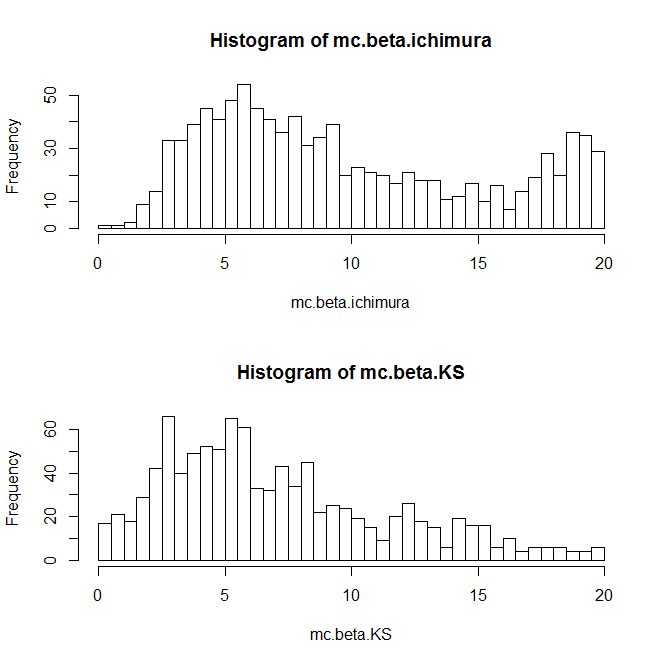
\includegraphics[width=0.6\linewidth]{30.png}
\end{figure}
\end{frame}

%------------------------------------------------

%------------------------------------------------

\begin{frame}
\frametitle{n = 100}
\begin{figure}
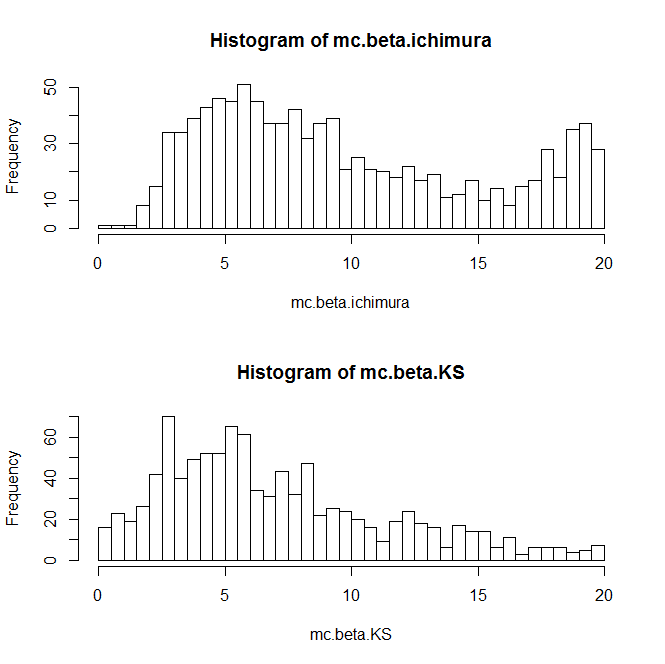
\includegraphics[width=0.6\linewidth]{100.png}
\end{figure}
\end{frame}



 \begin{frame}[t]
	\frametitle{Monte Carlo Simulation: comparison based on loss function}

\begin{table}
\begin{tabular}{l l l}
\toprule
\textbf{Number observations} & \textbf{Ichimura} & \textbf{Klein and Spady}\\
\midrule
30 & 68.16583 & 38.60356 \\
100 & 67.99048 & 38.59288 \\
\bottomrule
\end{tabular}
\caption{Results for loss function}
\end{table}
	\note{~}
\end{frame}


\begin{frame}[t]
	\frametitle{Monte Carlo Simulation}

	\textbf{What we are going to do}
	\begin{itemize}
		\item Continuous data (for comparison of Ichimura vs OLS )
		\item Binary data (for comparison of Probit, Ichimura, Klein and Spady)
           \item Vary the true distribution $g$ (for comparison of Ichimura and Klein and Spady)
	\end{itemize}
	\textbf{What we leave out}
	\begin{itemize}
		\item Comparsion between $g$ and $ G_{-i} $
	\end{itemize}
	\note{~}
\end{frame}


\begin{frame}
	\frametitle{Application on Real Data}
	
	\textbf{Data Features}
	\begin{itemize}
		\item Binary outcome: (Male or Female Voice)
		\item Include at least one continuous variable
		\item Features of voice: frequency, spectral flatness, peak frequency etc
	\end{itemize}
	\textbf{Steps in Estimation}
	\begin{itemize}
		\item Separate data into:
		\begin{itemize}
			\item Training sample
			\item Prediction sample
		\end{itemize}
		\item Same range of independent variable 
		\item Training sample to estimate $\hat{\beta}$ and $G_{-i}$
		\item Use those estimates on prediction sample
		\item Define accuracy rate for evaluation
	\end{itemize}
	\note{~}
\end{frame}

\begin{frame}[allowframebreaks]
    \frametitle{References}
    \renewcommand{\bibfont}{\normalfont\footnotesize}
    \printbibliography
\end{frame}


\end{document} 